\documentclass[conference]{IEEEtran}

\usepackage{graphicx}
\usepackage{float}
\usepackage{booktabs}
\usepackage{array}
\usepackage{tabularx}
\usepackage{makecell}
\usepackage{cite}
\usepackage{hyperref}
\usepackage{caption}
\usepackage{subcaption}

\title{Credit Card Fraud Detection and Cross-Dataset Generalization\\
\large AI3013 Course Project Report}

\author{
    \IEEEauthorblockN{Group 7}\vspace{0.2cm}\\
    \IEEEauthorblockA{
        \begin{tabular}{lc}
            Heran YANG & 2430034085 \\
            Haoyang JING & 2430034034 \\
            Jiyan LUO & 2430034045 \\
            Yifei SUN & 2430034061 \\
            Sirui ZHU & 2430034102 \\
        \end{tabular}
    }
}

\begin{document}
\maketitle

\begin{abstract}
This paper presents a reproducible machine learning pipeline for credit card fraud detection under severe class imbalance. We implement Logistic Regression (LR), Gaussian Naive Bayes (GNB), and k-Nearest Neighbors (kNN) from scratch, and evaluate them with stratified cross-validation and external validation on a 2023 dataset. The experiments include threshold calibration, confusion-matrix analysis, and ablation studies. Results show that LR achieves the most robust precision-recall trade-off across data distributions, while kNN remains weak even after weighted voting and PCA-based variants.
\end{abstract}

\begin{IEEEkeywords}
Credit card fraud detection, imbalanced classification, from-scratch implementation, threshold optimization, model generalization
\end{IEEEkeywords}

\section{Introduction}
Credit card fraud detection is a typical high-impact and highly imbalanced binary classification task. In this context, relying on Accuracy alone is misleading because a model can ignore minority fraud samples and still obtain high scores. Therefore, this work prioritizes Recall, F1, and PR-AUC, and uses Precision, ROC-AUC, and Accuracy as supporting indicators. The project objective is to build a fully reproducible pipeline and compare model behavior under distribution shift.

\section{Related Work}
Prior fraud detection studies consistently emphasize class imbalance handling, threshold calibration, and cost-sensitive evaluation. In this project, we focus on educational and reproducibility goals: implementing classic models from scratch and analyzing their practical trade-offs under a unified protocol, rather than proposing a new architecture.

\section{Methodology}
\subsection{Datasets}
\begin{table}[H]
\centering
\caption{Dataset summary}
\label{tab:dataset_summary}
\resizebox{\columnwidth}{!}{
\begin{tabular}{lrrr}
\toprule
Dataset & Samples & Features & Label Distribution \\
\midrule
Main dataset & 284{,}807 & 31 & 0: 284{,}315 / 1: 492 \\
External validation dataset & 568{,}630 & 31 & 0: 284{,}315 / 1: 284{,}315 \\
\bottomrule
\end{tabular}
}
\end{table}

Main dataset source: \texttt{Credit Card Fraud Detection/creditcard.csv} \cite{project_dataset_main}.\\
External dataset source: \texttt{Credit Card Fraud Detection\_2023/creditcard\_2023.csv} \cite{project_dataset_2023}.

\subsection{Preprocessing and Leakage Control}
\begin{itemize}
  \item Missing-value check and duplicate-row analysis are performed before training.
  \item The identifier field (\texttt{id}) is removed from the external dataset.
  \item Standardization statistics are computed on training data only and reused for validation/test data.
  \item All models share the same split and metric pipeline for fair comparison.
\end{itemize}

\subsection{Model Implementations}
We implement three models from scratch:
\begin{itemize}
  \item Logistic Regression (weighted loss, gradient descent),
  \item Gaussian Naive Bayes,
  \item kNN (uniform and distance-weighted voting).
\end{itemize}

\subsection{Evaluation Protocol}
\begin{itemize}
  \item Main dataset: 5-fold stratified cross-validation.
  \item External validation: threshold calibrated on main data and transferred to external data.
  \item Core metrics: Recall, F1, PR-AUC.
  \item Supporting metrics: Precision, ROC-AUC, Accuracy.
  \item Fine-grained threshold scan: step size 0.01.
\end{itemize}

\section{Experimental Setup}
\subsection{Baseline Setting}
Baseline comparison uses unified features and preprocessing across LR and GNB. kNN is evaluated under practical computational constraints with stratified subsampling and chunked distance computation.

\subsection{Ablation and Advanced Analysis}
We evaluate deduplication choices, class-weight variants, threshold strategies, and kNN enhancements (distance weighting and PCA+kNN). We also perform LR coefficient-based feature importance analysis.

\section{Results}
\subsection{Baseline Model Comparison}
\begin{table}[H]
\centering
\caption{Baseline results (5-fold + external validation)}
\label{tab:baseline_results}
\resizebox{\columnwidth}{!}{
\begin{tabular}{lcccccc}
\toprule
Model & Main Recall & Main F1 & Main PR-AUC & Ext Recall & Ext F1 & Ext PR-AUC \\
\midrule
Logistic Regression & 0.8605 & 0.4428 & 0.7116 & 0.8466 & 0.6949 & 0.7469 \\
Gaussian Naive Bayes & 0.8435 & 0.1092 & 0.4090 & 0.7974 & 0.6411 & 0.4939 \\
kNN & 0.8068 & 0.5811 & 0.6695 & 0.0274 & 0.0518 & 0.5051 \\
\bottomrule
\end{tabular}
}
\end{table}

\subsection{Fine-Grained Threshold Optimization (LR)}
Selected threshold on main data (step 0.01): \textbf{0.87}.
\begin{itemize}
  \item External Precision = 0.5913
  \item External Recall = 0.8339
  \item External F1 = 0.6920
  \item External Accuracy = 0.6288
\end{itemize}

\begin{figure}[H]
\centering
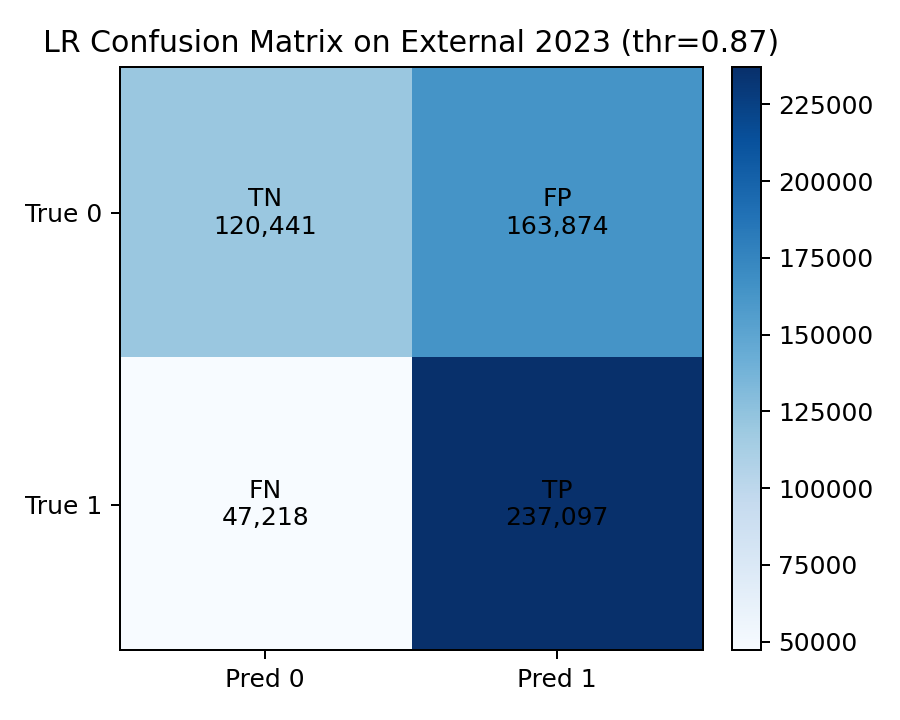
\includegraphics[width=\columnwidth]{figures/lr_confusion_matrix_ext2023_thr087.png}
\caption{LR confusion matrix on external dataset (threshold = 0.87)}
\label{fig:confusion_matrix_ext}
\end{figure}

\begin{figure}[H]
\centering
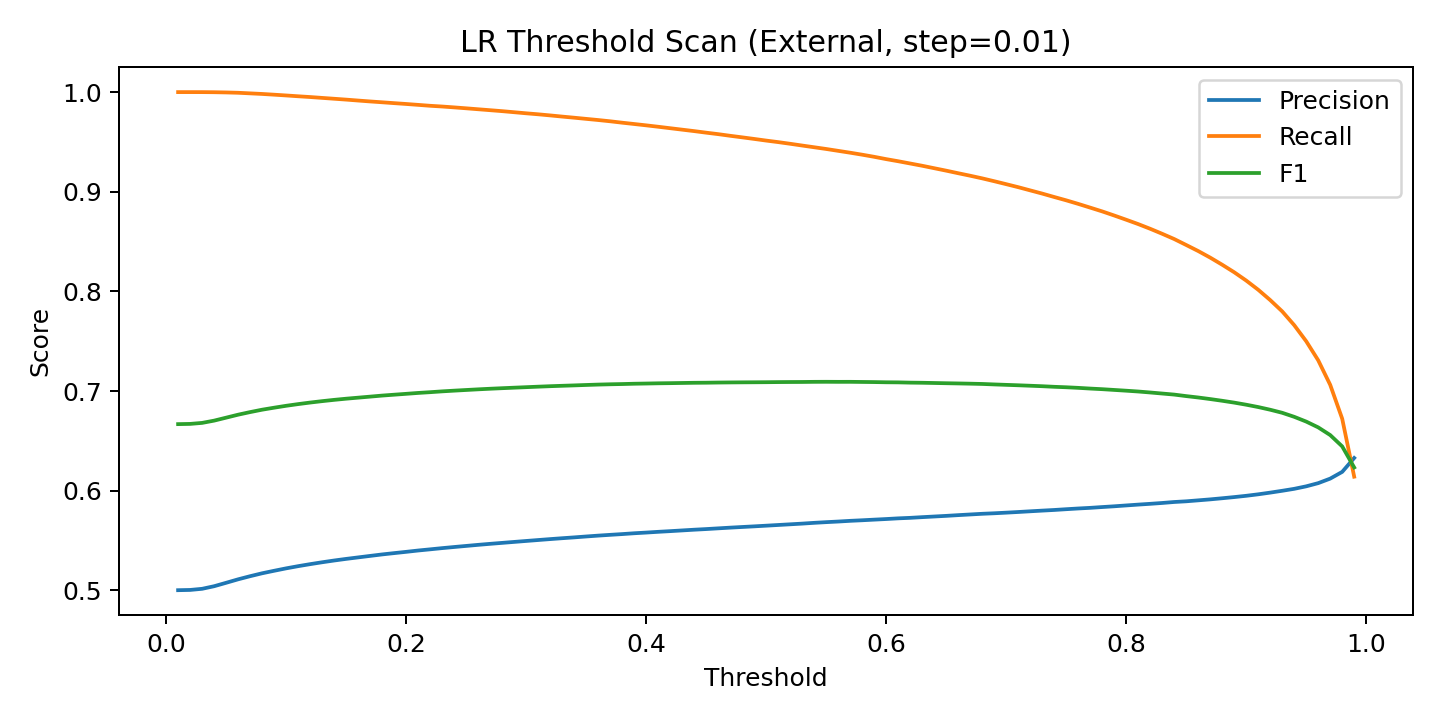
\includegraphics[width=\columnwidth]{figures/lr_threshold_scan_ext_001.png}
\caption{LR threshold scan on external dataset (step = 0.01)}
\label{fig:threshold_scan_ext}
\end{figure}

\subsection{Cost-Sensitive Threshold Analysis}
To align threshold selection with business risk, we define a cost objective:
\[
\text{Cost} = c_{fp}\cdot FP + c_{fn}\cdot FN
\]
and evaluate three settings: $1{:}5$, $1{:}10$, and $1{:}20$ for $c_{fp}{:}c_{fn}$.

\begin{table}[H]
\centering
\caption{Cost-sensitive threshold selection (selected on main, evaluated on external)}
\label{tab:cost_sensitive}
\resizebox{\columnwidth}{!}{
\begin{tabular}{lcccc}
\toprule
FP:FN Cost & Threshold & Ext Precision & Ext Recall & Ext F1 \\
\midrule
1:5  & 0.97 & 0.6121 & 0.7063 & 0.6558 \\
1:10 & 0.97 & 0.6121 & 0.7063 & 0.6558 \\
1:20 & 0.90 & 0.5949 & 0.8109 & 0.6863 \\
\bottomrule
\end{tabular}
}
\end{table}

\begin{figure}[H]
\centering
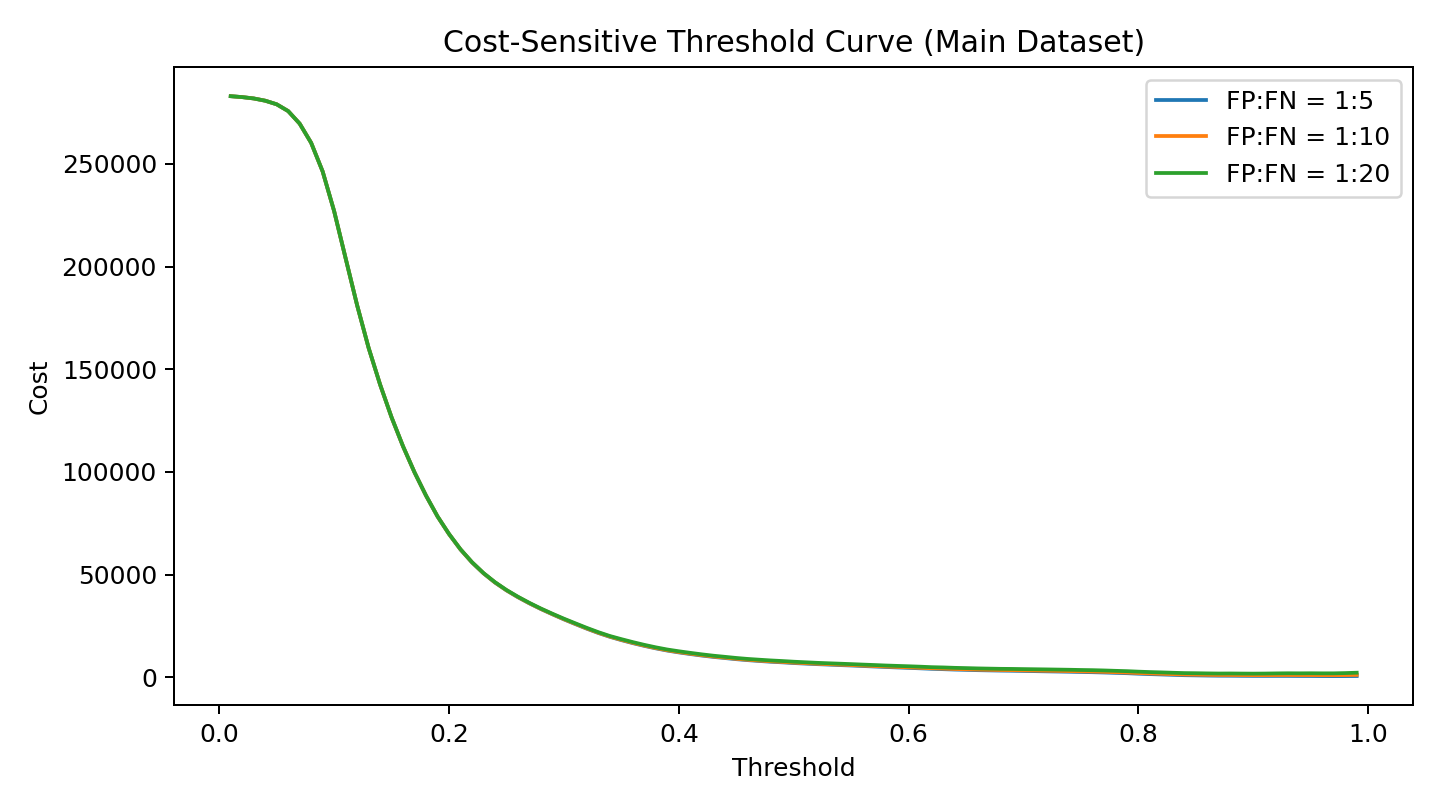
\includegraphics[width=\columnwidth]{figures/cost_curve_main.png}
\caption{Cost-sensitive threshold curves on main dataset}
\label{fig:cost_curve_main}
\end{figure}

\begin{figure}[H]
\centering
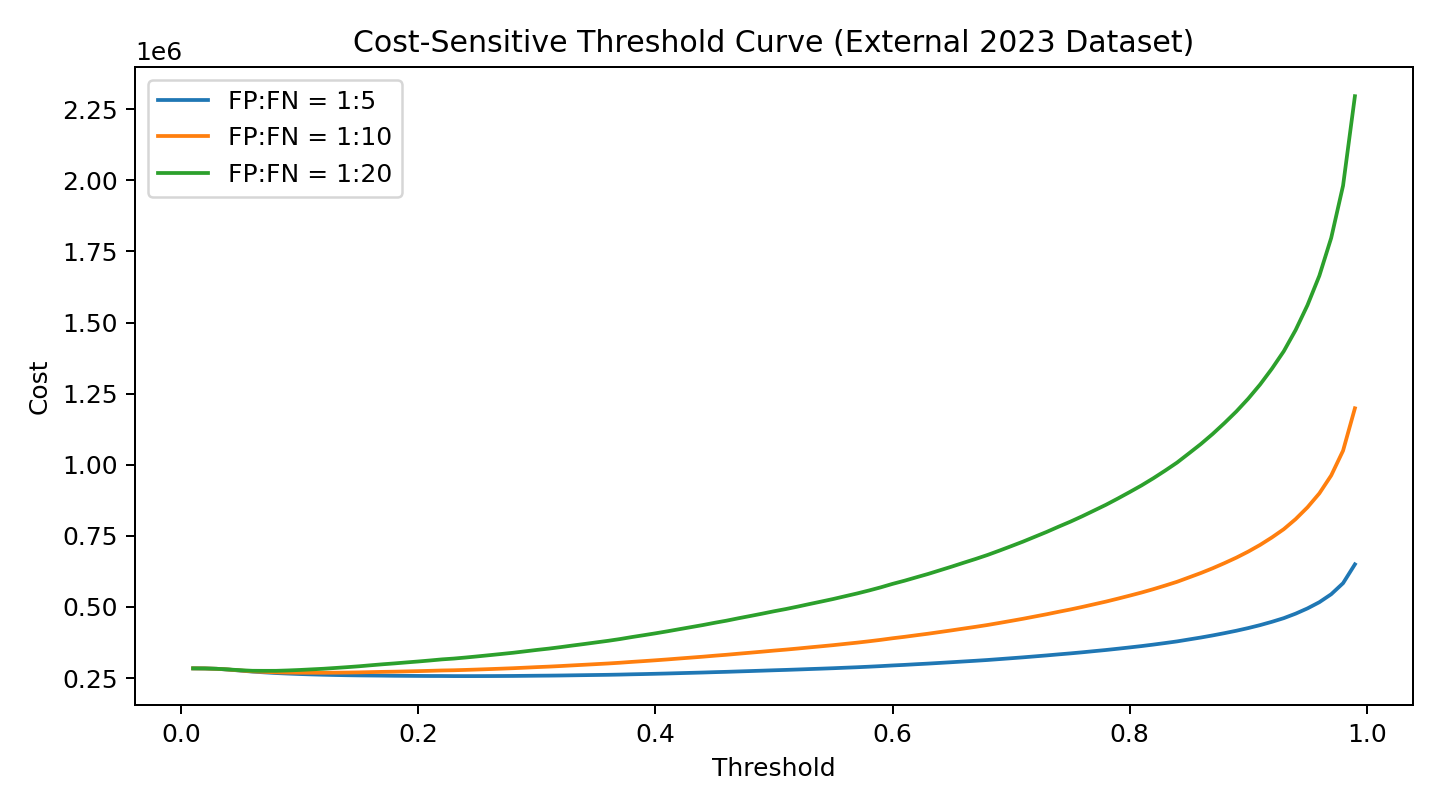
\includegraphics[width=\columnwidth]{figures/cost_curve_ext2023.png}
\caption{Cost-sensitive threshold curves on external dataset}
\label{fig:cost_curve_ext}
\end{figure}

When false-negative risk is heavily penalized ($1{:}20$), the selected threshold decreases from 0.97 to 0.90, which increases external recall from 0.7063 to 0.8109 while keeping competitive F1.

\subsection{Ablation Results}
\begin{table}[H]
\centering
\caption{Ablation results on external dataset}
\label{tab:ablation_results}
\resizebox{\columnwidth}{!}{
\begin{tabular}{lcccc}
\toprule
Setting & F1\_ext & Recall\_ext & Precision\_ext & Threshold \\
\midrule
dedup\_low\_pos\_weight & 0.7218 & 0.8110 & 0.6502 & 0.70 \\
no\_dedup\_auto\_weight & 0.6977 & 0.8343 & 0.5996 & 0.85 \\
baseline\_dedup\_auto\_weight & 0.6974 & 0.8382 & 0.5971 & 0.85 \\
dedup\_high\_pos\_weight & 0.6960 & 0.8618 & 0.5838 & 0.90 \\
dedup\_with\_amount\_raw & 0.6873 & 0.8840 & 0.5622 & 0.85 \\
\bottomrule
\end{tabular}
}
\end{table}

\subsection{Feature Importance (LR)}
\begin{figure}[H]
\centering
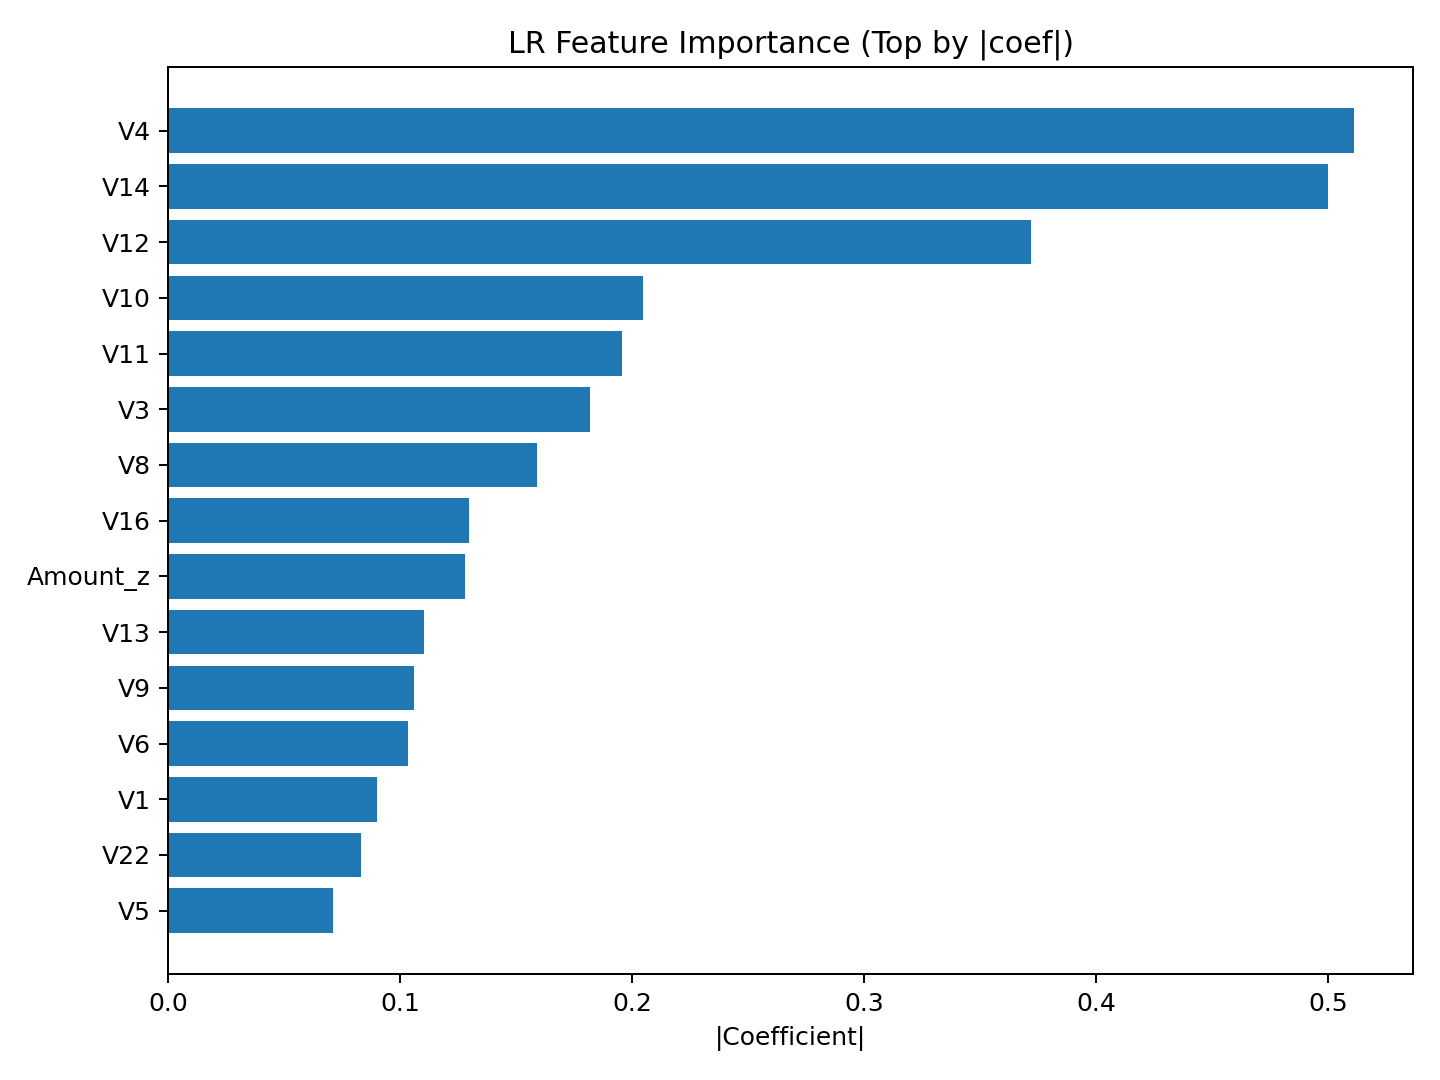
\includegraphics[width=\columnwidth]{figures/lr_feature_importance_top15.png}
\caption{LR feature importance (Top 15 by absolute coefficient)}
\label{fig:lr_feature_importance}
\end{figure}

Top influential features are \texttt{V4}, \texttt{V14}, \texttt{V12}, \texttt{V10}, and \texttt{V11}, indicating that a small subset of transformed variables dominates discriminative power.

\subsection{Temporal Robustness}
We perform an expanding-window chronological evaluation on the main dataset by splitting transactions into five time windows and testing on windows W2--W5. The threshold is re-calibrated on each training window.

\begin{table}[H]
\centering
\caption{Temporal robustness (expanding-window evaluation)}
\label{tab:temporal_robustness}
\resizebox{\columnwidth}{!}{
\begin{tabular}{ccccc}
\toprule
Window & Threshold & Precision & Recall & F1 \\
\midrule
W2 & 0.95 & 0.9500 & 0.7215 & 0.8201 \\
W3 & 0.94 & 0.6197 & 0.8302 & 0.7097 \\
W4 & 0.92 & 0.3719 & 0.7895 & 0.5056 \\
W5 & 0.89 & 0.4444 & 0.8108 & 0.5742 \\
\bottomrule
\end{tabular}
}
\end{table}

\begin{figure}[H]
\centering
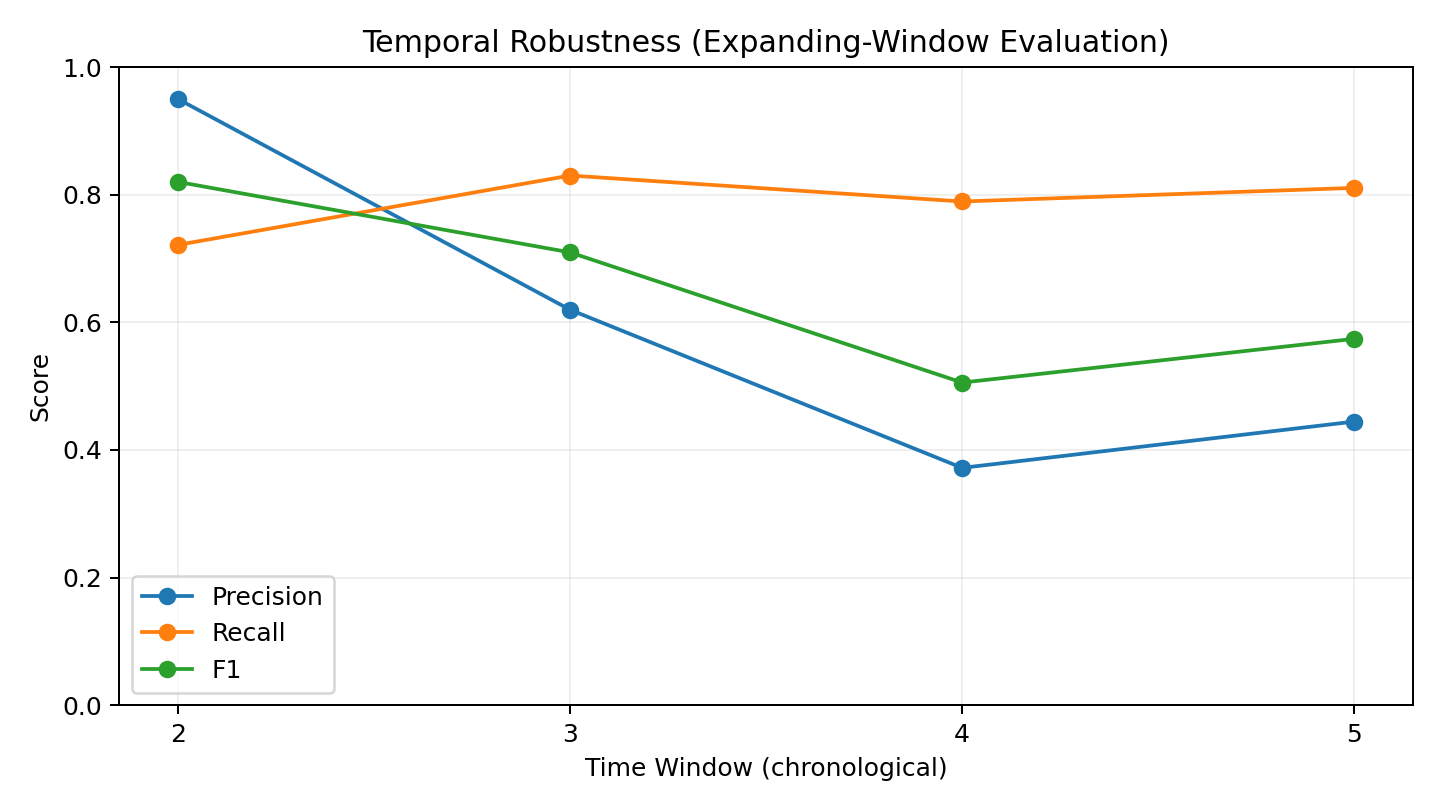
\includegraphics[width=\columnwidth]{figures/temporal_robustness_metrics.png}
\caption{Precision/Recall/F1 across chronological windows}
\label{fig:temporal_robustness}
\end{figure}

\begin{figure}[H]
\centering
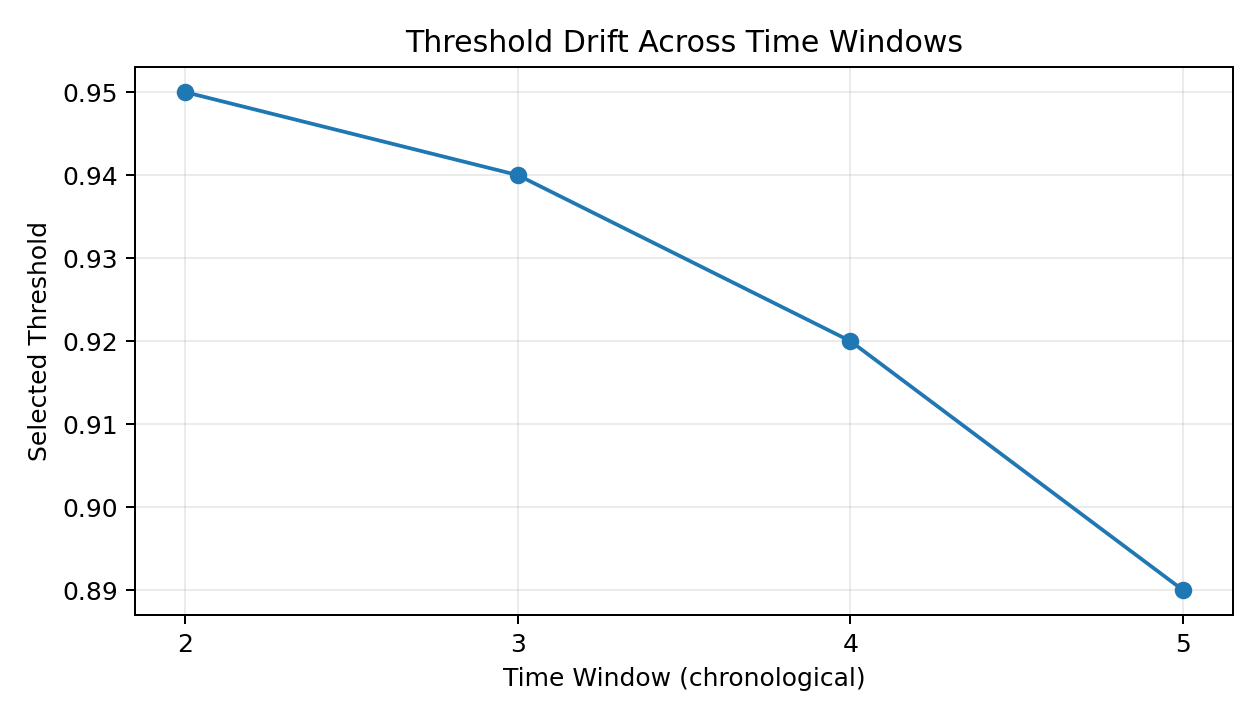
\includegraphics[width=\columnwidth]{figures/temporal_threshold_drift.png}
\caption{Threshold drift across chronological windows}
\label{fig:temporal_threshold_drift}
\end{figure}

The temporal results show moderate performance drift (F1 standard deviation: 0.1215). Thresholds also drift from 0.95 to 0.89, suggesting periodic recalibration is necessary for stable deployment.

\subsection{Error Analysis}
We further analyze prediction errors on the external dataset under the selected LR threshold of 0.87. The case distribution is:
\[
TP=237097,\quad FP=163874,\quad FN=47218,\quad TN=120441
\]
This result indicates that the current operating point still produces a large number of false alarms, even though fraud coverage remains high.

\begin{figure}[H]
\centering
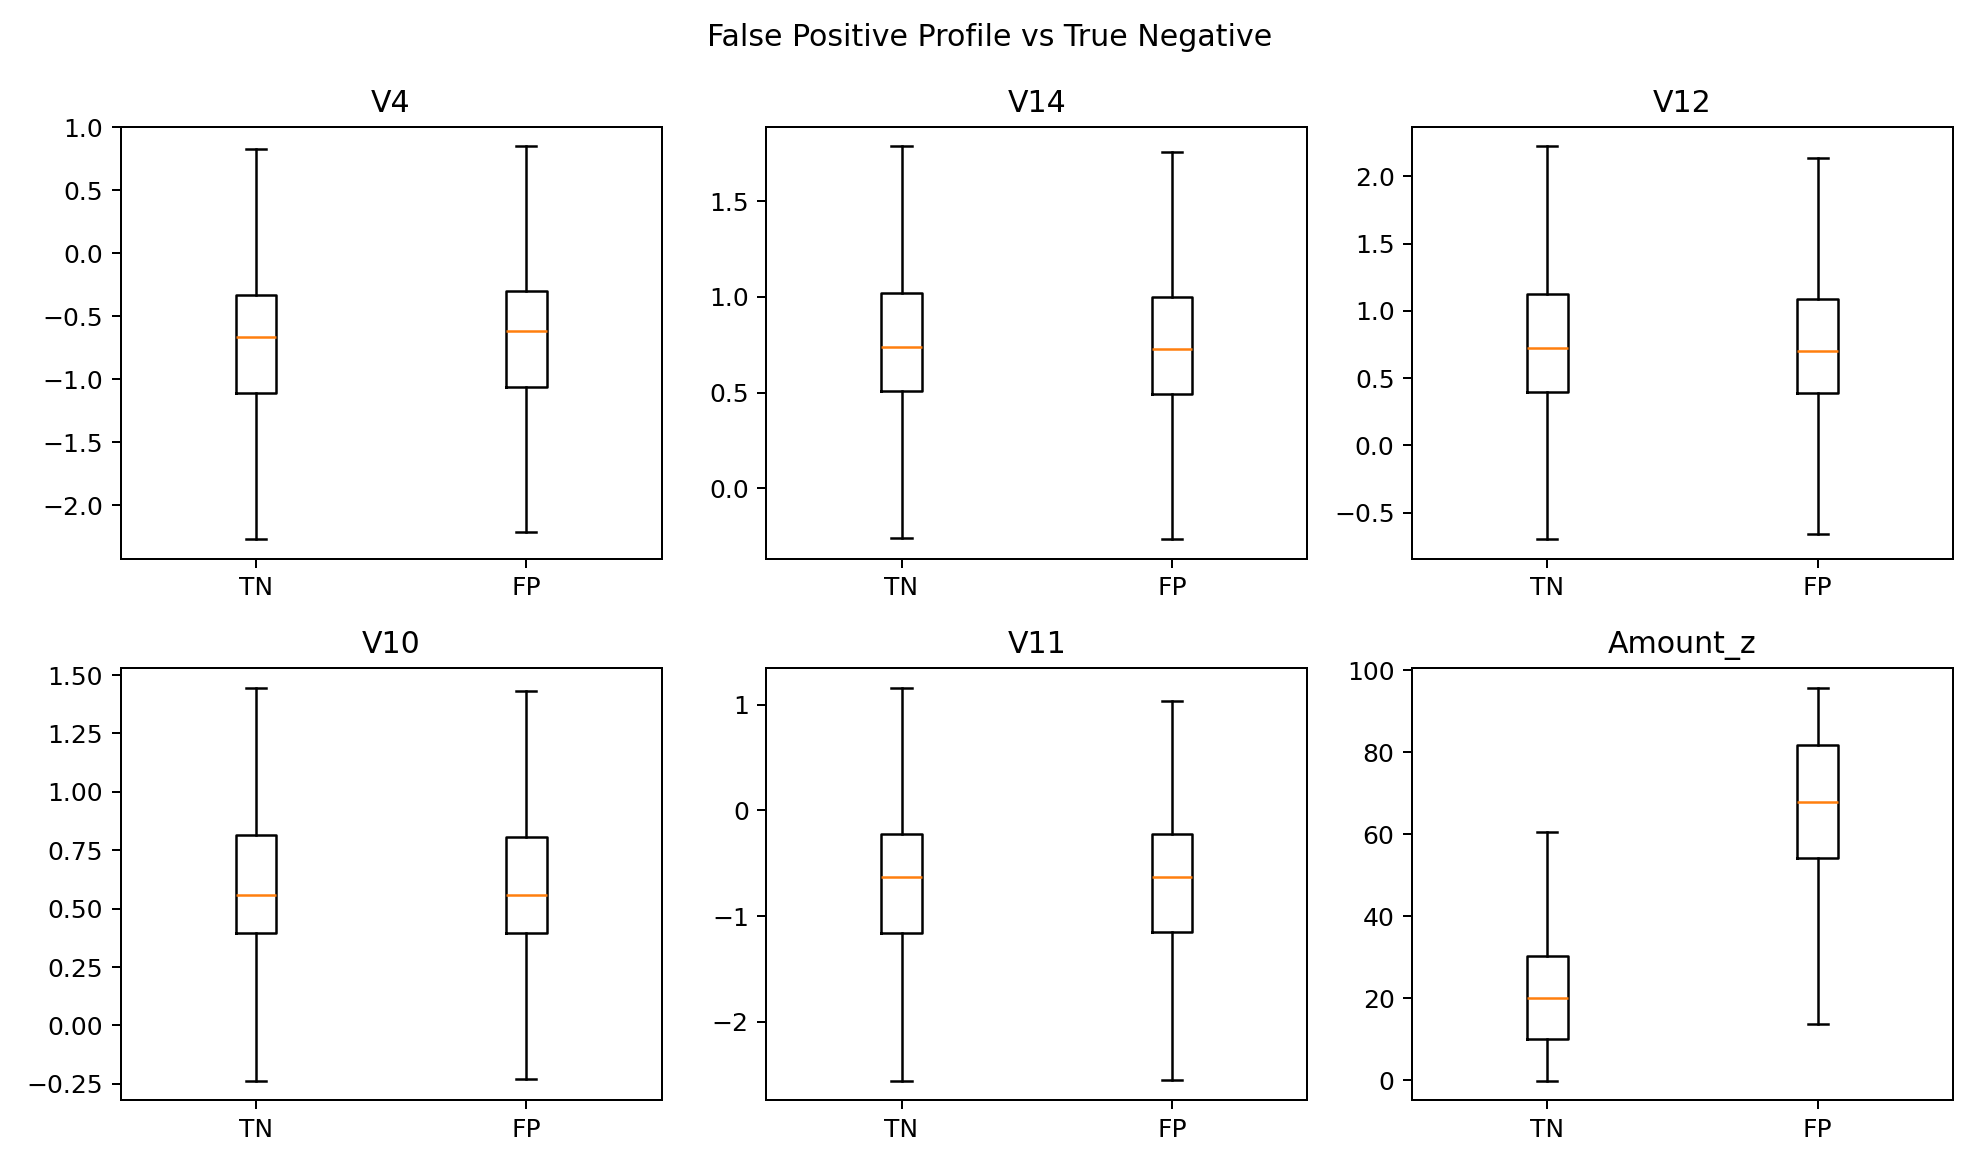
\includegraphics[width=\columnwidth]{figures/error_profile_fp_vs_tn.png}
\caption{Feature profile comparison between false positives and true negatives}
\label{fig:error_fp_tn}
\end{figure}

\begin{figure}[H]
\centering
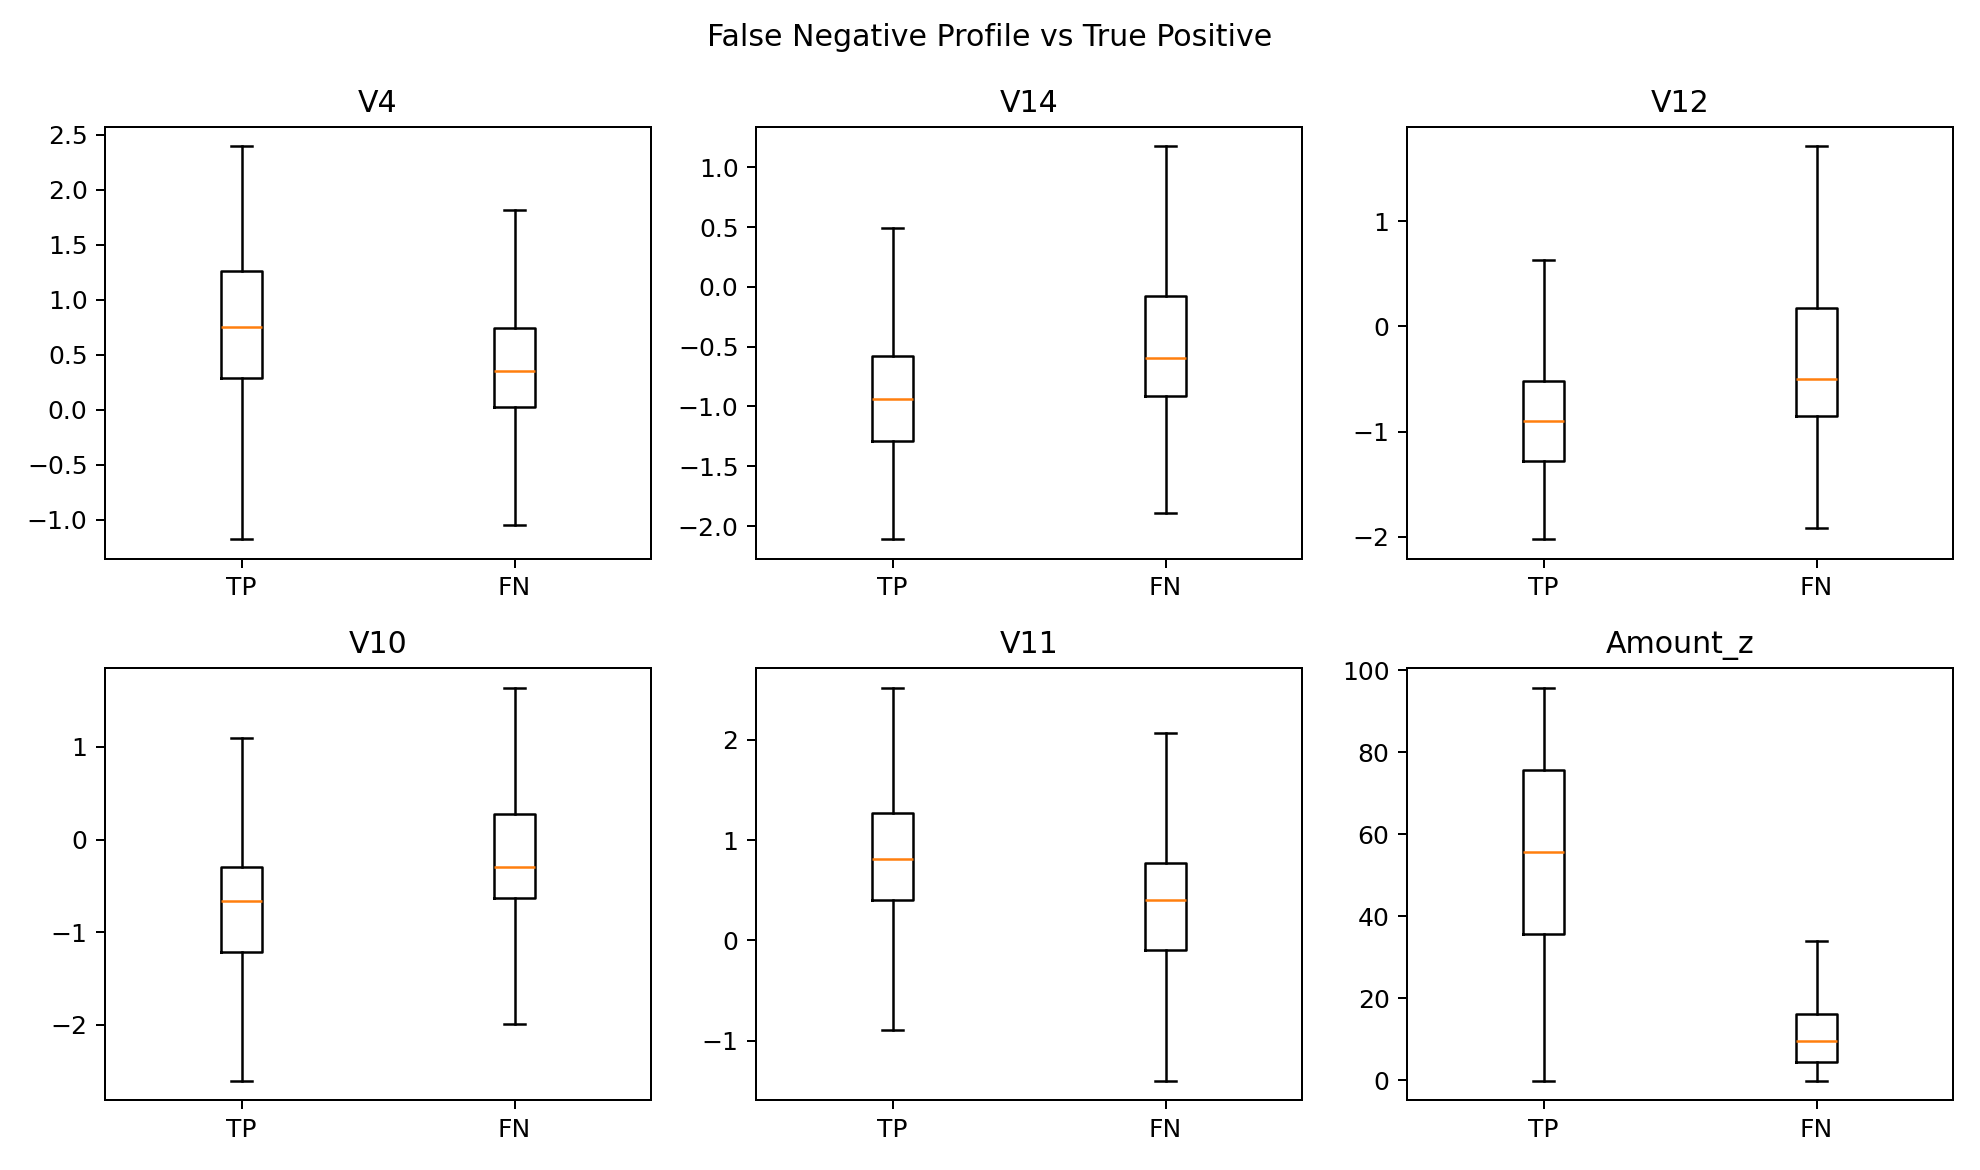
\includegraphics[width=\columnwidth]{figures/error_profile_fn_vs_tp.png}
\caption{Feature profile comparison between false negatives and true positives}
\label{fig:error_fn_tp}
\end{figure}

The most obvious false-positive shift appears on \texttt{Amount\_z}, where FP samples are substantially larger than TN samples on average. For false negatives, the largest deviations relative to true positives occur on \texttt{V10} and \texttt{V11}, suggesting that missed fraud samples are less extreme on these discriminative variables and are therefore harder to separate from normal transactions. These observations suggest two practical directions: adding more targeted amount-related controls for false-positive reduction, and strengthening feature interactions around \texttt{V10}/\texttt{V11} to improve fraud recall without excessive alarm inflation.

\subsection{Notebook-Inspired Extensions}
We reviewed two reference notebooks and integrated their useful ideas as controlled project extensions rather than replacing the core from-scratch pipeline. The adopted components include richer external-data EDA, preprocessing sensitivity checks, and non-core mature-library benchmarks.

\begin{figure}[H]
\centering
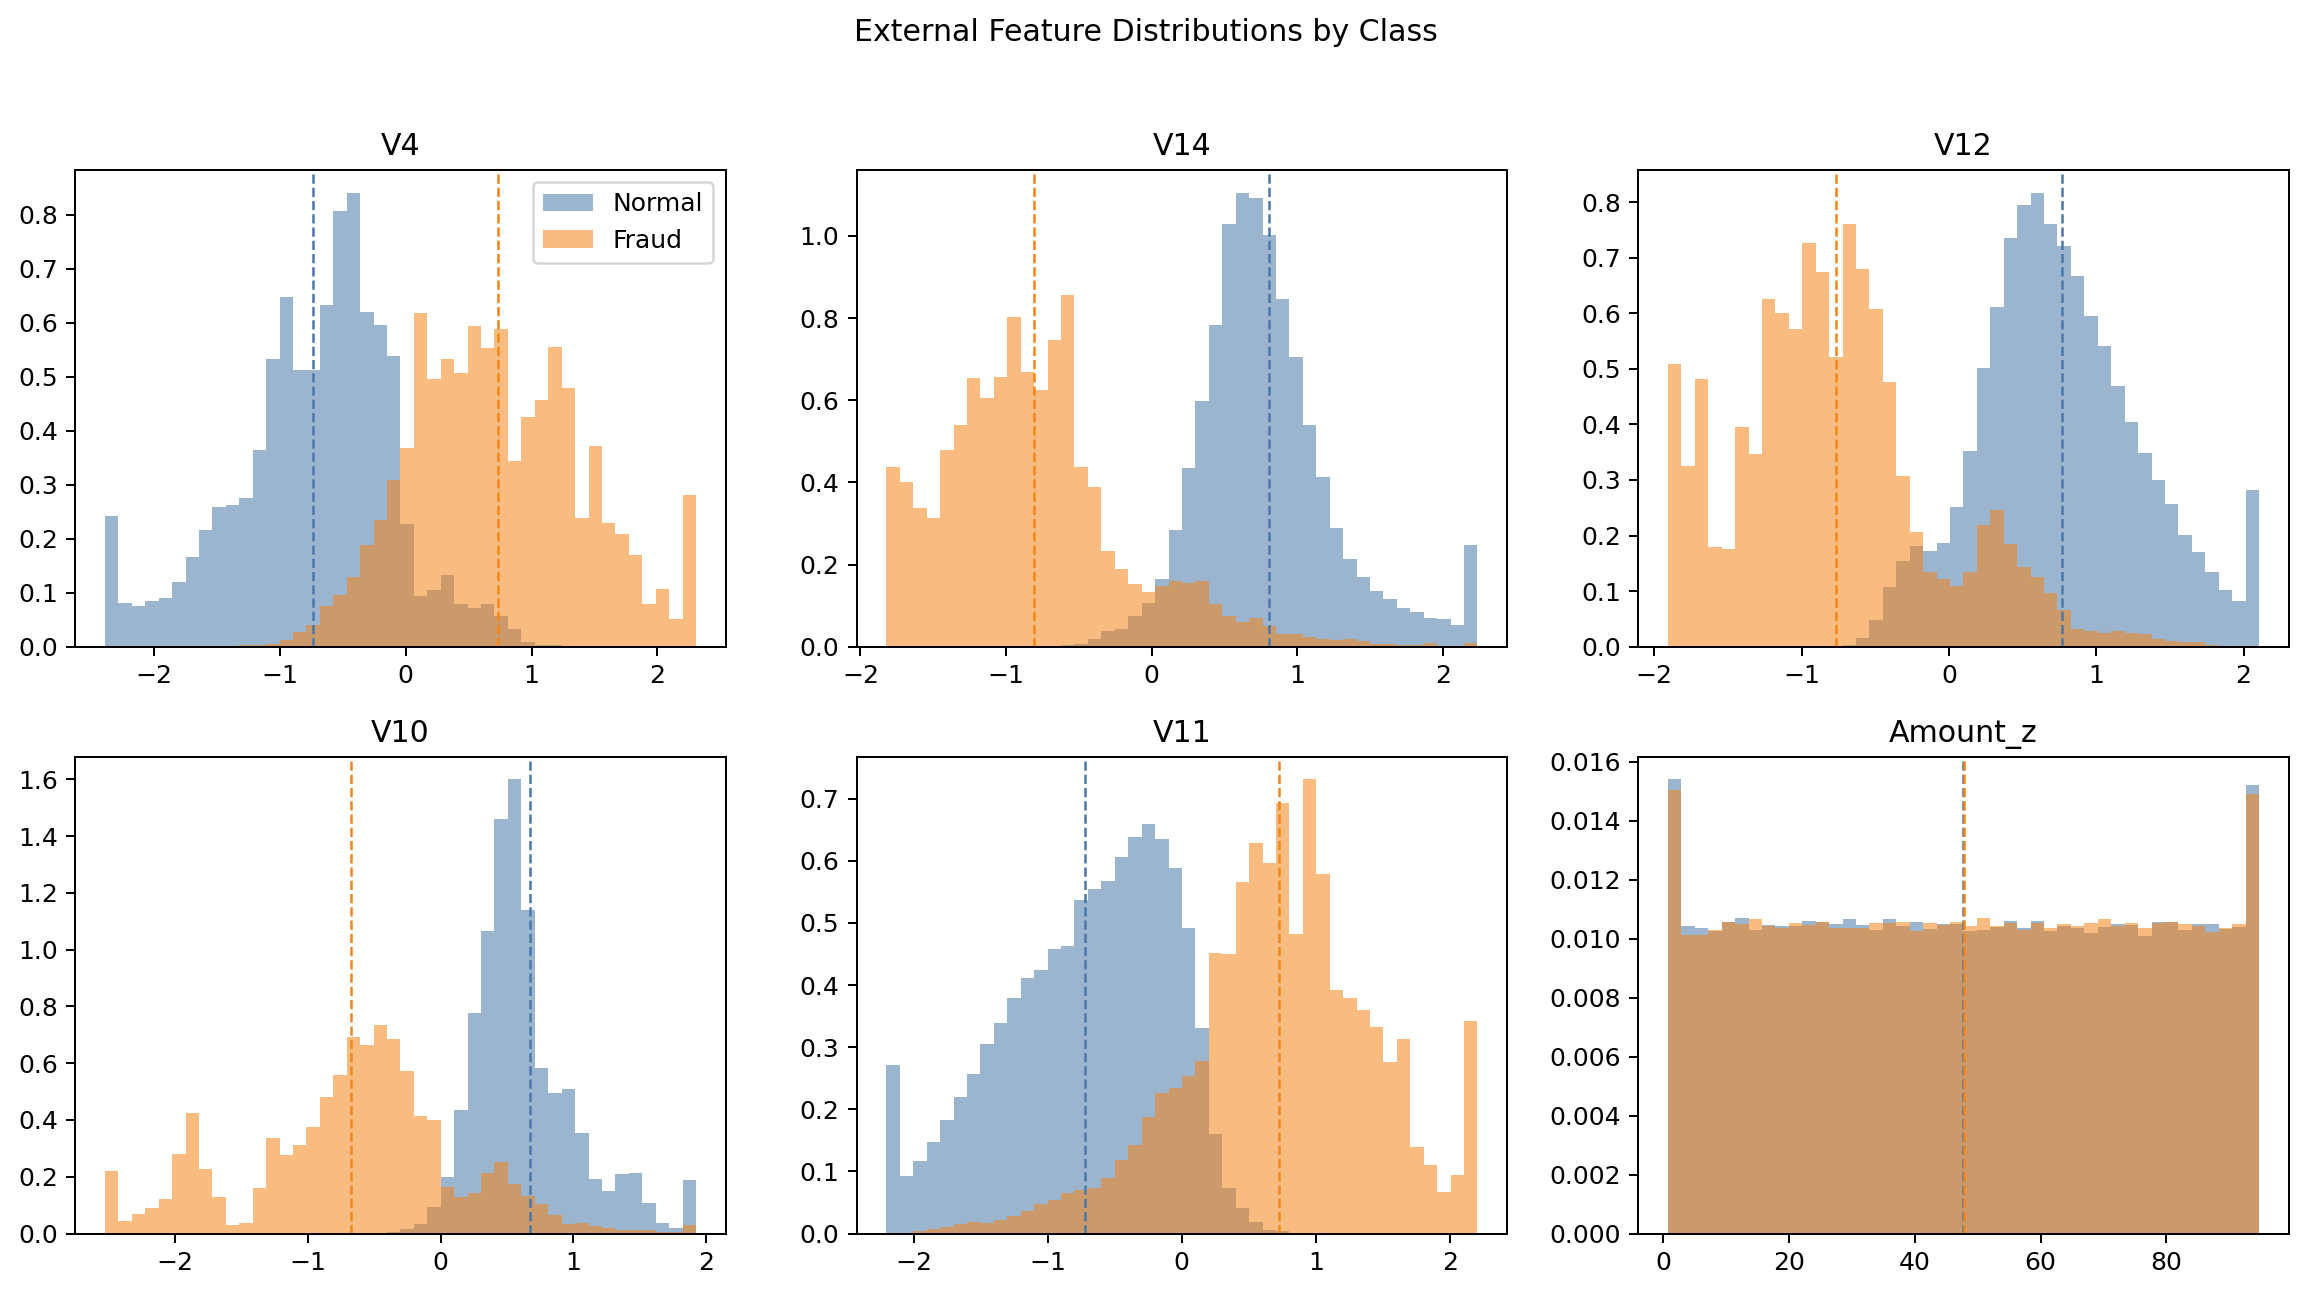
\includegraphics[width=\columnwidth]{figures/external_feature_histograms_by_class.png}
\caption{External 2023 feature distributions by class, inspired by notebook EDA}
\label{fig:external_histograms}
\end{figure}

The external EDA confirms that \texttt{V14}, \texttt{V12}, \texttt{V4}, \texttt{V11}, and \texttt{V10} are among the features most correlated with the fraud label. This aligns with the LR feature-importance result and provides additional evidence that a small group of transformed variables drives most discrimination.

\begin{table}[H]
\centering
\caption{Scaling ablation inspired by notebook preprocessing}
\label{tab:scaling_ablation}
\resizebox{\columnwidth}{!}{
\begin{tabular}{llcccc}
\toprule
Model & Scaler & Precision & Recall & F1 & PR-AUC \\
\midrule
LR & standard & 0.5949 & 0.8394 & 0.6963 & 0.7545 \\
LR & min-max & 0.9995 & 0.7693 & 0.8694 & 0.9634 \\
LR & robust & 0.9916 & 0.0058 & 0.0116 & 0.8075 \\
kNN & standard & 0.8000 & 0.0016 & 0.0032 & 0.5012 \\
kNN & min-max & 0.8095 & 0.0068 & 0.0135 & 0.5077 \\
kNN & robust & 1.0000 & 0.0010 & 0.0020 & 0.5014 \\
\bottomrule
\end{tabular}
}
\end{table}

\begin{figure}[H]
\centering
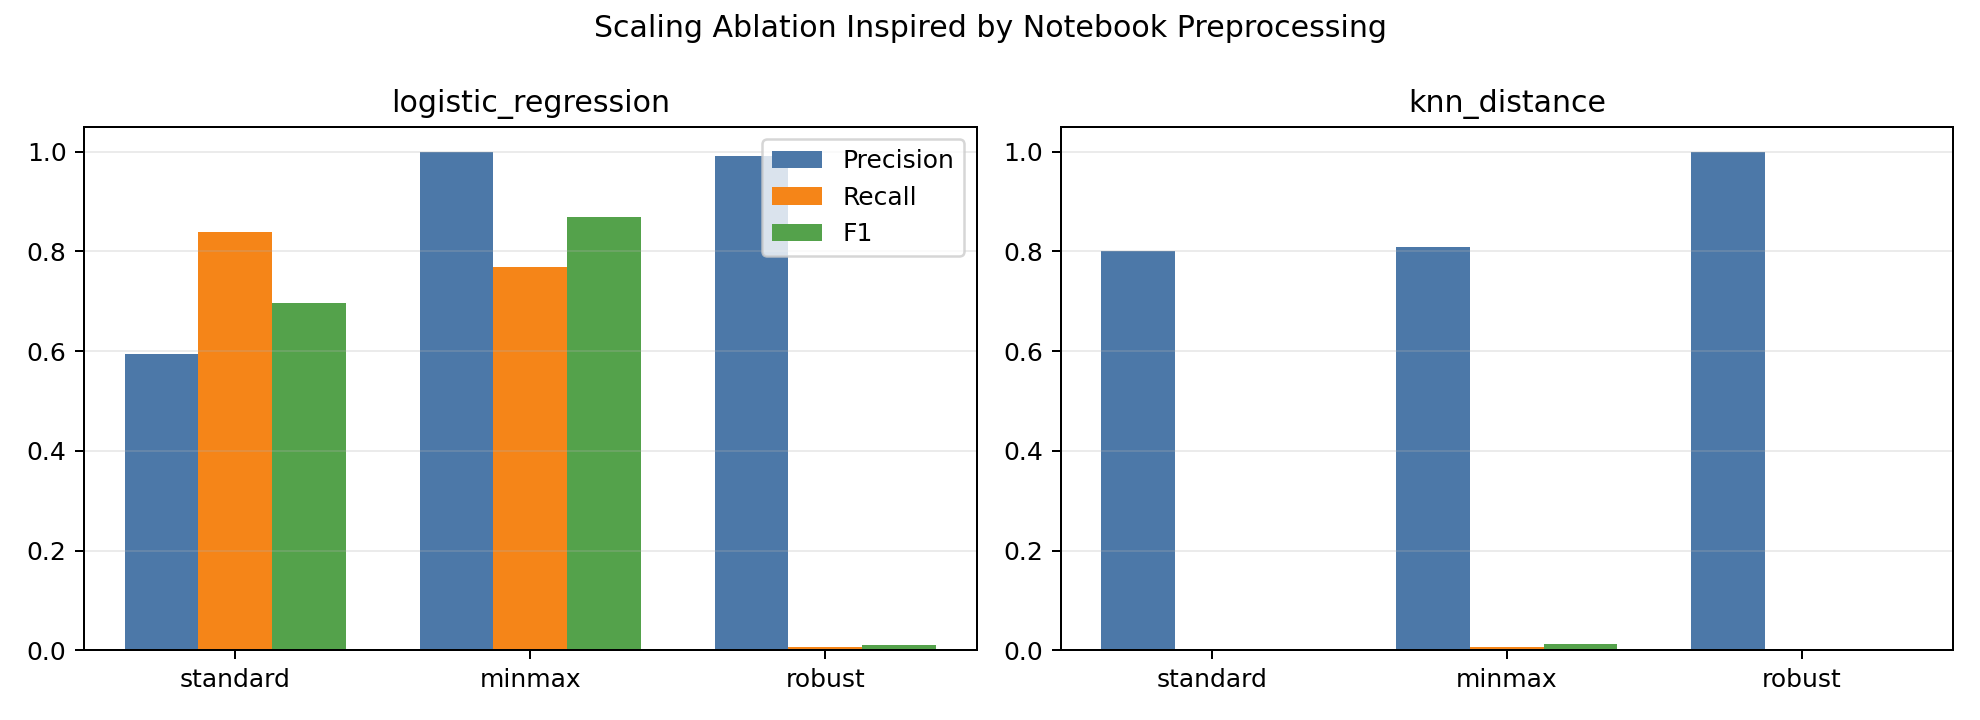
\includegraphics[width=\columnwidth]{figures/scaling_ablation_compare.png}
\caption{Scaling ablation comparison for from-scratch LR and kNN}
\label{fig:scaling_ablation}
\end{figure}

The scaling study shows that preprocessing has a strong effect on LR calibration and external transfer. Min-max scaling gives the strongest external F1 in this extension, while kNN remains weak regardless of scaling. Because this is an additional sensitivity experiment, the main report keeps the standard-scaling baseline as the primary comparable setting and treats min-max scaling as a promising follow-up configuration.

\begin{table}[H]
\centering
\caption{Mature library benchmark (non-core reference)}
\label{tab:library_benchmark}
\resizebox{\columnwidth}{!}{
\begin{tabular}{lcccc}
\toprule
Model & Precision & Recall & F1 & PR-AUC \\
\midrule
sklearn Logistic Regression & 0.5103 & 0.9848 & 0.6722 & 0.3737 \\
HistGradientBoosting & 1.0000 & 0.0566 & 0.1072 & 0.9255 \\
Random Forest & 1.0000 & 0.0001 & 0.0001 & 0.9402 \\
\bottomrule
\end{tabular}
}
\end{table}

\begin{figure}[H]
\centering
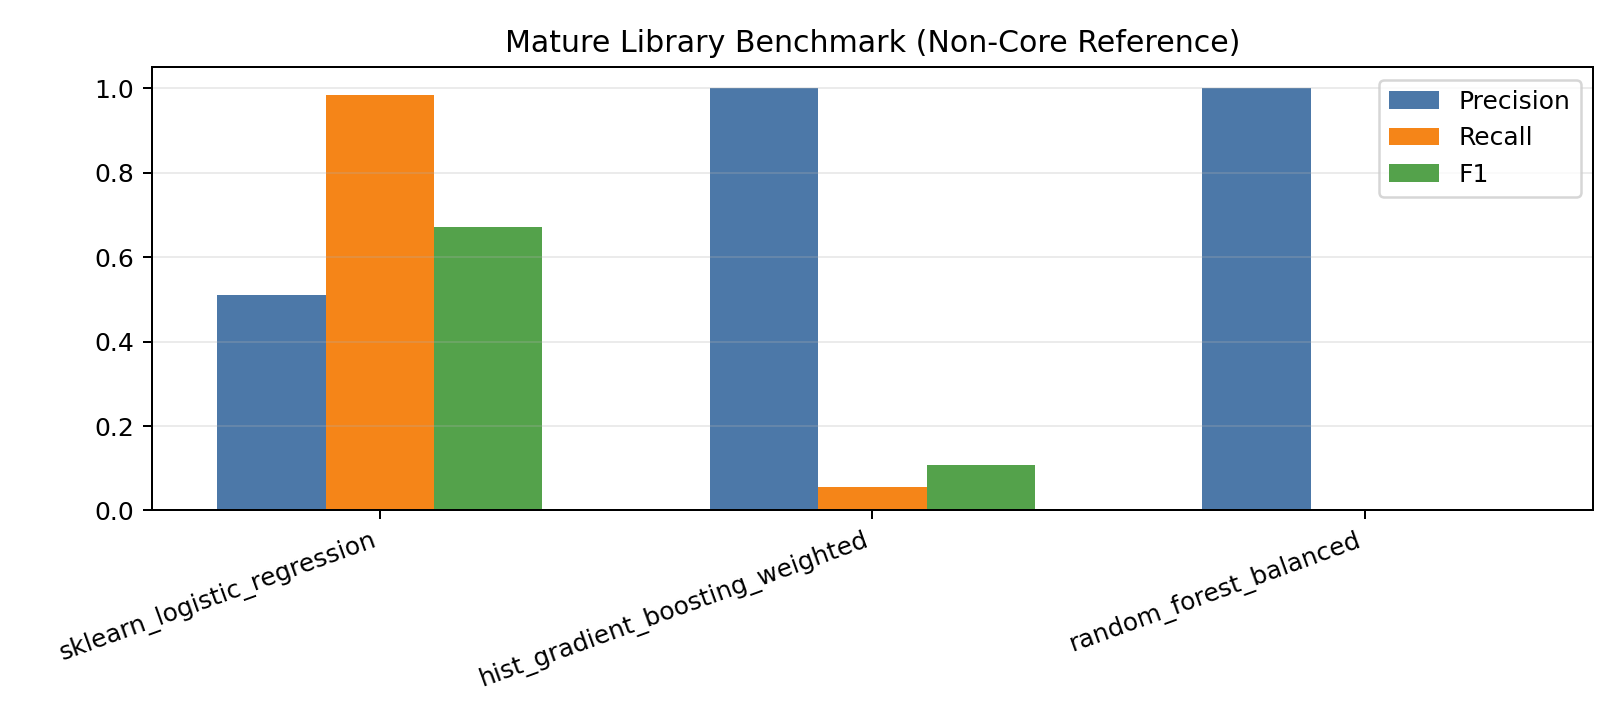
\includegraphics[width=\columnwidth]{figures/library_benchmark_compare.png}
\caption{Mature library benchmark as a non-core reference}
\label{fig:library_benchmark}
\end{figure}

These mature-library results are intentionally reported as reference only. They show that tree-based models can rank external cases well by PR-AUC, but transferring a main-data threshold still produces poor recall. This supports the project's emphasis on threshold calibration and cross-dataset validation instead of relying on same-distribution accuracy.

\subsection{OOF Threshold and MinMax Mainline Review}
To reduce optimistic bias from selecting thresholds on full in-sample main-data scores, we add a 5-fold out-of-fold (OOF) threshold-selection experiment. The threshold is selected from OOF scores on the main dataset, then transferred to the full external 2023 dataset.

\begin{table}[H]
\centering
\caption{OOF-selected threshold transfer to external dataset}
\label{tab:oof_minmax}
\resizebox{\columnwidth}{!}{
\begin{tabular}{lccccc}
\toprule
Scaler & OOF Threshold & Ext Precision & Ext Recall & Ext F1 & Ext PR-AUC \\
\midrule
standard & 0.85 & 0.5894 & 0.8466 & 0.6949 & 0.7469 \\
min-max & 0.41 & 0.9996 & 0.5695 & 0.7256 & 0.9640 \\
\bottomrule
\end{tabular}
}
\end{table}

\begin{figure}[H]
\centering
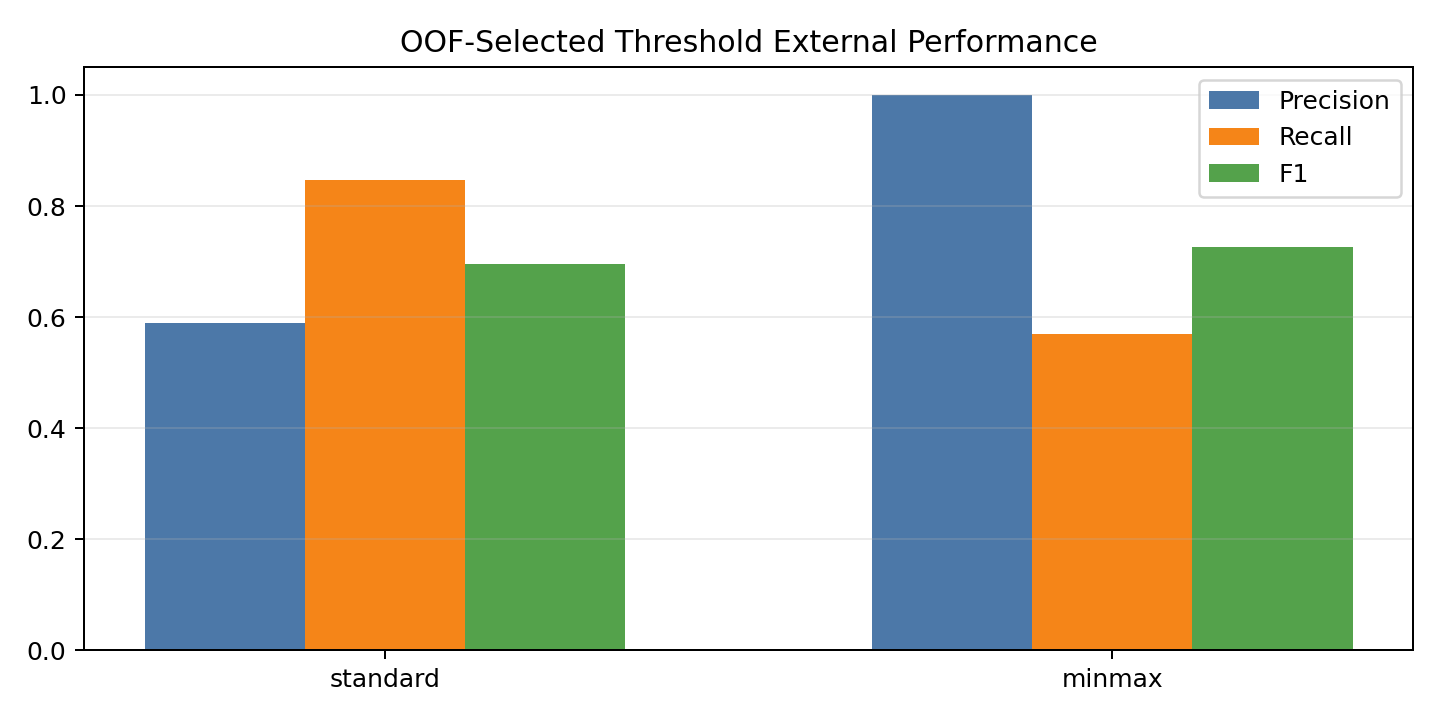
\includegraphics[width=\columnwidth]{figures/oof_minmax_external_compare.png}
\caption{External performance using thresholds selected from OOF predictions}
\label{fig:oof_minmax_compare}
\end{figure}

The stricter OOF review changes the interpretation of the MinMax result. MinMax still improves external F1 and nearly eliminates false positives (FP = 59), but recall falls to 0.5695. Therefore, MinMax is best treated as a low-false-alarm strategy, while the standard-scaling LR remains the safer high-recall baseline.

\section{Discussion}
The experiments show that LR provides the best overall robustness under both imbalance and distribution shift. GNB is computationally efficient but significantly weaker in PR-AUC and F1. kNN variants remain underperforming in this setting, even with distance weighting and PCA, suggesting limited suitability for large-scale fraud detection with current feature space and class ratios.

\section{Conclusion}
This work delivers a complete from-scratch pipeline for fraud detection with reproducible scripts, unified evaluation, and cross-dataset validation. LR is selected as the primary model due to consistently strong precision-recall performance. Future work includes finer threshold policies under explicit cost constraints and targeted false-positive reduction.

\bibliographystyle{IEEEtran}
\bibliography{refs/references}

\end{document}
